\documentclass[1p]{elsarticle_modified}
%\bibliographystyle{elsarticle-num}

%\usepackage[colorlinks]{hyperref}
%\usepackage{abbrmath_seonhwa} %\Abb, \Ascr, \Acal ,\Abf, \Afrak
\usepackage{amsfonts}
\usepackage{amssymb}
\usepackage{amsmath}
\usepackage{amsthm}
\usepackage{scalefnt}
\usepackage{amsbsy}
\usepackage{kotex}
\usepackage{caption}
\usepackage{subfig}
\usepackage{color}
\usepackage{graphicx}
\usepackage{xcolor} %% white, black, red, green, blue, cyan, magenta, yellow
\usepackage{float}
\usepackage{setspace}
\usepackage{hyperref}

\usepackage{tikz}
\usetikzlibrary{arrows}

\usepackage{multirow}
\usepackage{array} % fixed length table
\usepackage{hhline}

%%%%%%%%%%%%%%%%%%%%%
\makeatletter
\renewcommand*\env@matrix[1][\arraystretch]{%
	\edef\arraystretch{#1}%
	\hskip -\arraycolsep
	\let\@ifnextchar\new@ifnextchar
	\array{*\c@MaxMatrixCols c}}
\makeatother %https://tex.stackexchange.com/questions/14071/how-can-i-increase-the-line-spacing-in-a-matrix
%%%%%%%%%%%%%%%

\usepackage[normalem]{ulem}

\newcommand{\msout}[1]{\ifmmode\text{\sout{\ensuremath{#1}}}\else\sout{#1}\fi}
%SOURCE: \msout is \stkout macro in https://tex.stackexchange.com/questions/20609/strikeout-in-math-mode

\newcommand{\cancel}[1]{
	\ifmmode
	{\color{red}\msout{#1}}
	\else
	{\color{red}\sout{#1}}
	\fi
}

\newcommand{\add}[1]{
	{\color{blue}\uwave{#1}}
}

\newcommand{\replace}[2]{
	\ifmmode
	{\color{red}\msout{#1}}{\color{blue}\uwave{#2}}
	\else
	{\color{red}\sout{#1}}{\color{blue}\uwave{#2}}
	\fi
}

\newcommand{\Sol}{\mathcal{S}} %segment
\newcommand{\D}{D} %diagram
\newcommand{\A}{\mathcal{A}} %arc


%%%%%%%%%%%%%%%%%%%%%%%%%%%%%5 test

\def\sl{\operatorname{\textup{SL}}(2,\Cbb)}
\def\psl{\operatorname{\textup{PSL}}(2,\Cbb)}
\def\quan{\mkern 1mu \triangleright \mkern 1mu}

\theoremstyle{definition}
\newtheorem{thm}{Theorem}[section]
\newtheorem{prop}[thm]{Proposition}
\newtheorem{lem}[thm]{Lemma}
\newtheorem{ques}[thm]{Question}
\newtheorem{cor}[thm]{Corollary}
\newtheorem{defn}[thm]{Definition}
\newtheorem{exam}[thm]{Example}
\newtheorem{rmk}[thm]{Remark}
\newtheorem{alg}[thm]{Algorithm}

\newcommand{\I}{\sqrt{-1}}
\begin{document}

%\begin{frontmatter}
%
%\title{Boundary parabolic representations of knots up to 8 crossings}
%
%%% Group authors per affiliation:
%\author{Yunhi Cho} 
%\address{Department of Mathematics, University of Seoul, Seoul, Korea}
%\ead{yhcho@uos.ac.kr}
%
%
%\author{Seonhwa Kim} %\fnref{s_kim}}
%\address{Center for Geometry and Physics, Institute for Basic Science, Pohang, 37673, Korea}
%\ead{ryeona17@ibs.re.kr}
%
%\author{Hyuk Kim}
%\address{Department of Mathematical Sciences, Seoul National University, Seoul 08826, Korea}
%\ead{hyukkim@snu.ac.kr}
%
%\author{Seokbeom Yoon}
%\address{Department of Mathematical Sciences, Seoul National University, Seoul, 08826,  Korea}
%\ead{sbyoon15@snu.ac.kr}
%
%\begin{abstract}
%We find all boundary parabolic representation of knots up to 8 crossings.
%
%\end{abstract}
%\begin{keyword}
%    \MSC[2010] 57M25 
%\end{keyword}
%
%\end{frontmatter}

%\linenumbers
%\tableofcontents
%
\newcommand\colored[1]{\textcolor{white}{\rule[-0.35ex]{0.8em}{1.4ex}}\kern-0.8em\color{red} #1}%
%\newcommand\colored[1]{\textcolor{white}{ #1}\kern-2.17ex	\textcolor{white}{ #1}\kern-1.81ex	\textcolor{white}{ #1}\kern-2.15ex\color{red}#1	}

{\Large $\underline{11a_{281}~(K11a_{281})}$}

\setlength{\tabcolsep}{10pt}
\renewcommand{\arraystretch}{1.6}
\vspace{1cm}\begin{tabular}{m{100pt}>{\centering\arraybackslash}m{274pt}}
\multirow{5}{120pt}{
	\centering
	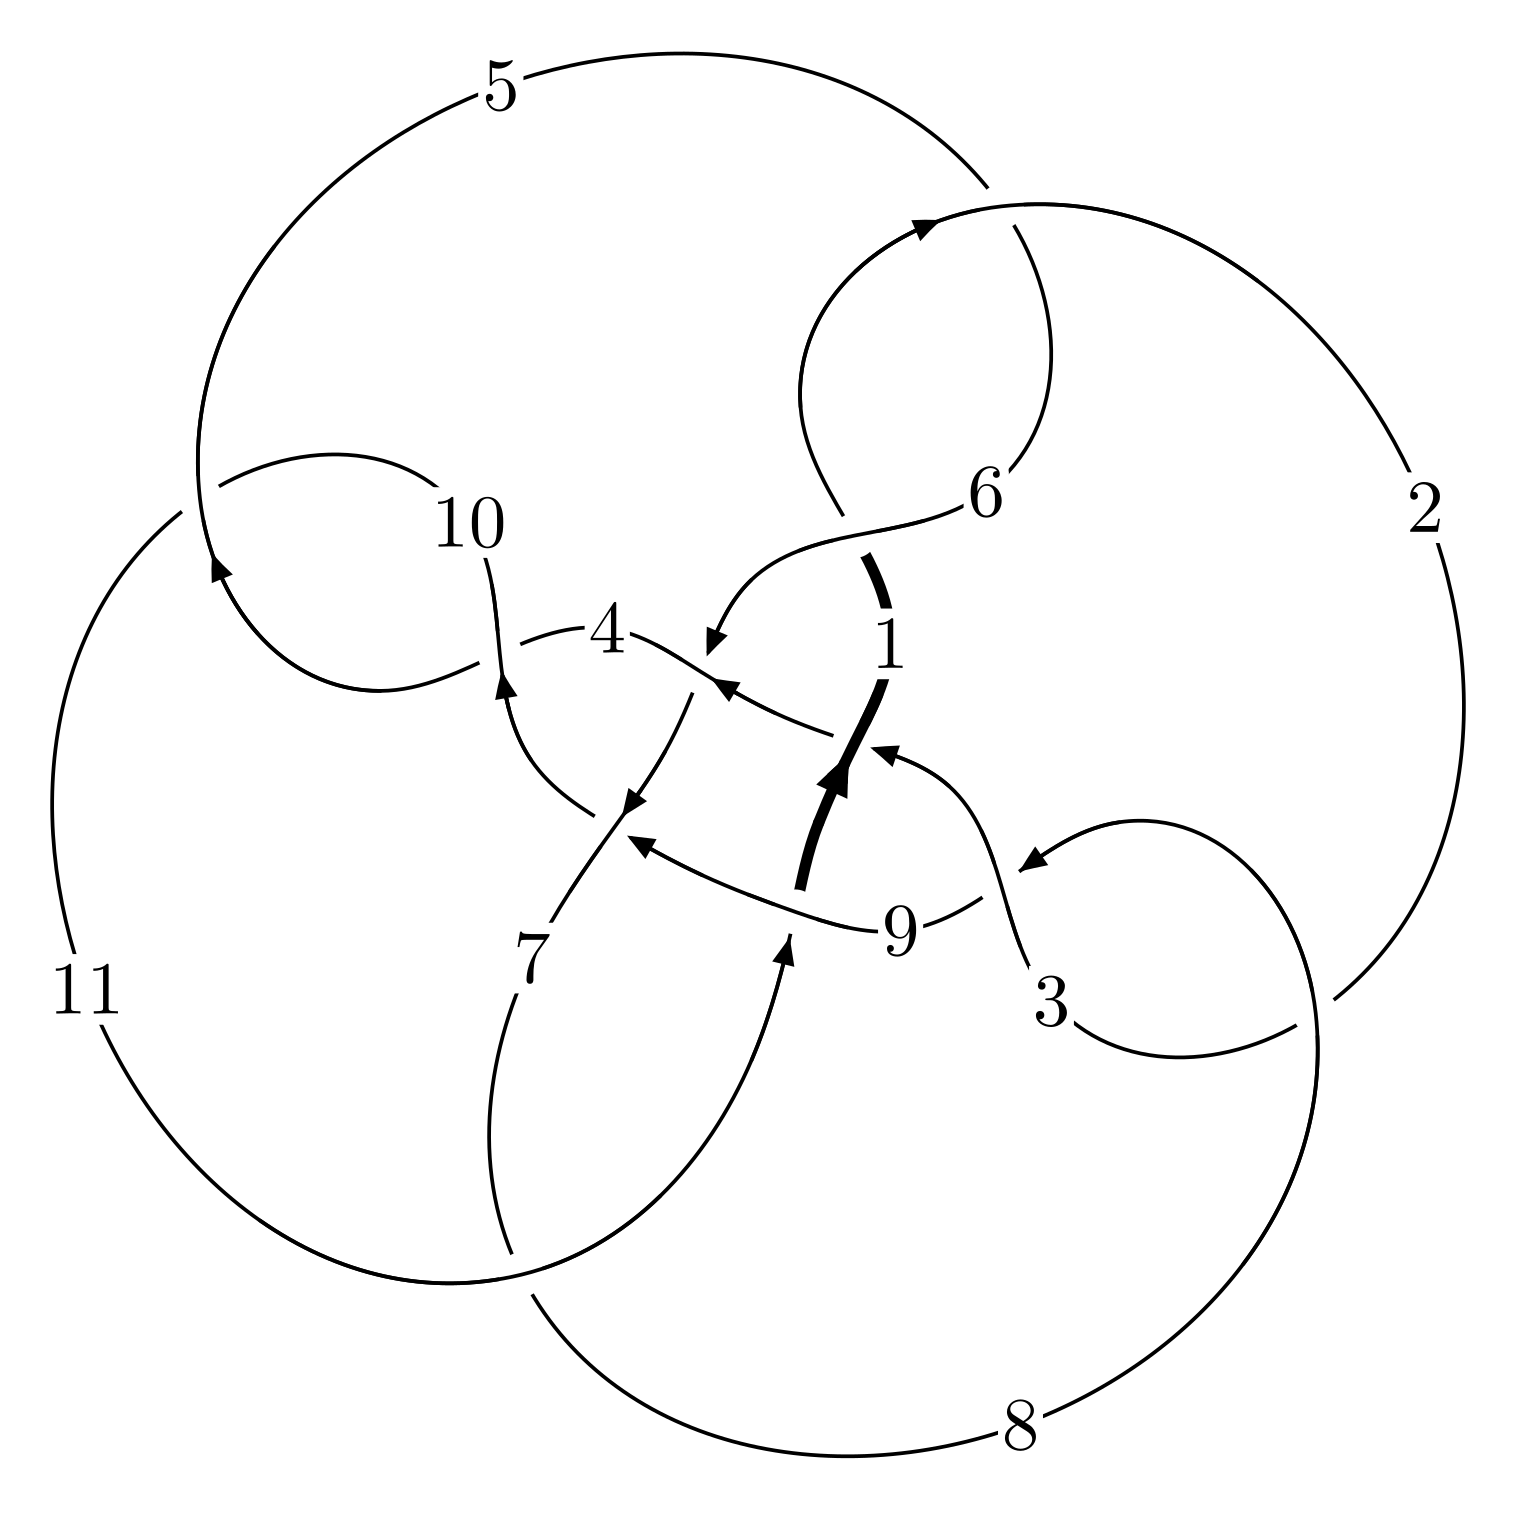
\includegraphics[width=112pt]{../../../GIT/diagram.site/Diagrams/png/530_11a_281.png}\\
\ \ \ A knot diagram\footnotemark}&
\allowdisplaybreaks
\textbf{Linearized knot diagam} \\
\cline{2-2}
 &
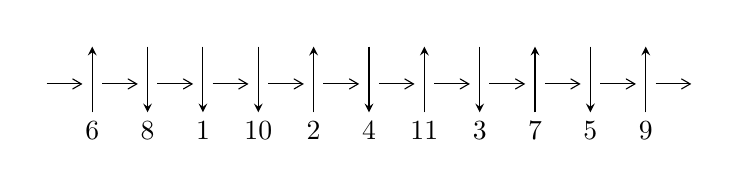
\begin{tikzpicture}[x=20pt, y=17pt]
	% nodes
	\node (C0) at (0, 0) {};
	\node (C1) at (1, 0) {};
	\node (C1U) at (1, +1) {};
	\node (C1D) at (1, -1) {6};

	\node (C2) at (2, 0) {};
	\node (C2U) at (2, +1) {};
	\node (C2D) at (2, -1) {8};

	\node (C3) at (3, 0) {};
	\node (C3U) at (3, +1) {};
	\node (C3D) at (3, -1) {1};

	\node (C4) at (4, 0) {};
	\node (C4U) at (4, +1) {};
	\node (C4D) at (4, -1) {10};

	\node (C5) at (5, 0) {};
	\node (C5U) at (5, +1) {};
	\node (C5D) at (5, -1) {2};

	\node (C6) at (6, 0) {};
	\node (C6U) at (6, +1) {};
	\node (C6D) at (6, -1) {4};

	\node (C7) at (7, 0) {};
	\node (C7U) at (7, +1) {};
	\node (C7D) at (7, -1) {11};

	\node (C8) at (8, 0) {};
	\node (C8U) at (8, +1) {};
	\node (C8D) at (8, -1) {3};

	\node (C9) at (9, 0) {};
	\node (C9U) at (9, +1) {};
	\node (C9D) at (9, -1) {7};

	\node (C10) at (10, 0) {};
	\node (C10U) at (10, +1) {};
	\node (C10D) at (10, -1) {5};

	\node (C11) at (11, 0) {};
	\node (C11U) at (11, +1) {};
	\node (C11D) at (11, -1) {9};
	\node (C12) at (12, 0) {};

	% arrows
	\draw[->,>={angle 60}]
	(C0) edge (C1) (C1) edge (C2) (C2) edge (C3) (C3) edge (C4) (C4) edge (C5) (C5) edge (C6) (C6) edge (C7) (C7) edge (C8) (C8) edge (C9) (C9) edge (C10) (C10) edge (C11) (C11) edge (C12) ;	\draw[->,>=stealth]
	(C1D) edge (C1U) (C2U) edge (C2D) (C3U) edge (C3D) (C4U) edge (C4D) (C5D) edge (C5U) (C6U) edge (C6D) (C7D) edge (C7U) (C8U) edge (C8D) (C9D) edge (C9U) (C10U) edge (C10D) (C11D) edge (C11U) ;
	\end{tikzpicture} \\
\hhline{~~} \\& 
\textbf{Solving Sequence} \\ \cline{2-2} 
 &
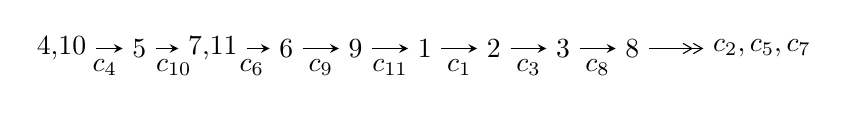
\begin{tikzpicture}[x=25pt, y=7pt]
	% node
	\node (A0) at (-1/8, 0) {4,10};
	\node (A1) at (1, 0) {5};
	\node (A2) at (33/16, 0) {7,11};
	\node (A3) at (25/8, 0) {6};
	\node (A4) at (33/8, 0) {9};
	\node (A5) at (41/8, 0) {1};
	\node (A6) at (49/8, 0) {2};
	\node (A7) at (57/8, 0) {3};
	\node (A8) at (65/8, 0) {8};
	\node (C1) at (1/2, -1) {$c_{4}$};
	\node (C2) at (3/2, -1) {$c_{10}$};
	\node (C3) at (21/8, -1) {$c_{6}$};
	\node (C4) at (29/8, -1) {$c_{9}$};
	\node (C5) at (37/8, -1) {$c_{11}$};
	\node (C6) at (45/8, -1) {$c_{1}$};
	\node (C7) at (53/8, -1) {$c_{3}$};
	\node (C8) at (61/8, -1) {$c_{8}$};
	\node (A9) at (10, 0) {$c_{2},c_{5},c_{7}$};

	% edge
	\draw[->,>=stealth]	
	(A0) edge (A1) (A1) edge (A2) (A2) edge (A3) (A3) edge (A4) (A4) edge (A5) (A5) edge (A6) (A6) edge (A7) (A7) edge (A8) ;
	\draw[->>,>={angle 60}]	
	(A8) edge (A9);
\end{tikzpicture} \\ 

\end{tabular} \\

\footnotetext{
The image of knot diagram is generated by the software ``\textbf{Draw programme}" developed by Andrew Bartholomew(\url{http://www.layer8.co.uk/maths/draw/index.htm\#Running-draw}), where we modified some parts for our purpose(\url{https://github.com/CATsTAILs/LinksPainter}).
}\phantom \\ \newline 
\centering \textbf{Ideals for irreducible components\footnotemark of $X_{\text{par}}$} 
 
\begin{align*}
I^u_{1}&=\langle 
-41702317014899 u^{28}-43018944579853 u^{27}+\cdots+142344490041062 b-32762826071390,\\
\phantom{I^u_{1}}&\phantom{= \langle  }-214382018217017 u^{28}-235461945222166 u^{27}+\cdots+284688980082124 a+218463983805488,\\
\phantom{I^u_{1}}&\phantom{= \langle  }u^{29}-12 u^{27}+\cdots+4 u+4\rangle \\
I^u_{2}&=\langle 
1.20003\times10^{196} u^{67}+5.15521\times10^{196} u^{66}+\cdots+5.31191\times10^{195} b-8.00012\times10^{197},\\
\phantom{I^u_{2}}&\phantom{= \langle  }2.93592\times10^{198} u^{67}+1.24026\times10^{199} u^{66}+\cdots+1.06610\times10^{199} a-1.22115\times10^{200},\\
\phantom{I^u_{2}}&\phantom{= \langle  }3 u^{68}+16 u^{67}+\cdots-121 u-223\rangle \\
I^u_{3}&=\langle 
4170 u^{11}+9821 u^{10}+\cdots+1318 b-848,\;60429 u^{11}+266417 u^{10}+\cdots+23724 a-45544,\\
\phantom{I^u_{3}}&\phantom{= \langle  }3 u^{12}+5 u^{11}-3 u^{10}-15 u^9-10 u^8+16 u^7+45 u^6+35 u^5-15 u^4-36 u^3-10 u^2+8 u+4\rangle \\
I^u_{4}&=\langle 
- u^3+b+u,\;u^7- u^6-4 u^5+3 u^4+5 u^3- u^2+a-2 u-3,\;u^8-4 u^6+5 u^4+u^3- u^2-2 u-1\rangle \\
\\
\end{align*}
\raggedright * 4 irreducible components of $\dim_{\mathbb{C}}=0$, with total 117 representations.\\
\footnotetext{All coefficients of polynomials are rational numbers. But the coefficients are sometimes approximated in decimal forms when there is not enough margin.}
\newpage
\renewcommand{\arraystretch}{1}
\centering \section*{I. $I^u_{1}= \langle -4.17\times10^{13} u^{28}-4.30\times10^{13} u^{27}+\cdots+1.42\times10^{14} b-3.28\times10^{13},\;-2.14\times10^{14} u^{28}-2.35\times10^{14} u^{27}+\cdots+2.85\times10^{14} a+2.18\times10^{14},\;u^{29}-12 u^{27}+\cdots+4 u+4 \rangle$}
\flushleft \textbf{(i) Arc colorings}\\
\begin{tabular}{m{7pt} m{180pt} m{7pt} m{180pt} }
\flushright $a_{4}=$&$\begin{pmatrix}1\\0\end{pmatrix}$ \\
\flushright $a_{10}=$&$\begin{pmatrix}0\\u\end{pmatrix}$ \\
\flushright $a_{5}=$&$\begin{pmatrix}1\\u^2\end{pmatrix}$ \\
\flushright $a_{7}=$&$\begin{pmatrix}0.753039 u^{28}+0.827085 u^{27}+\cdots-5.75342 u-0.767378\\0.292968 u^{28}+0.302217 u^{27}+\cdots+0.399336 u+0.230166\end{pmatrix}$ \\
\flushright $a_{11}=$&$\begin{pmatrix}- u\\- u^3+u\end{pmatrix}$ \\
\flushright $a_{6}=$&$\begin{pmatrix}1.04601 u^{28}+1.12930 u^{27}+\cdots-5.35408 u-0.537212\\0.292968 u^{28}+0.302217 u^{27}+\cdots+0.399336 u+0.230166\end{pmatrix}$ \\
\flushright $a_{9}=$&$\begin{pmatrix}0.198212 u^{28}-0.192154 u^{27}+\cdots-3.96388 u+2.24602\\0.345416 u^{28}+0.736164 u^{27}+\cdots-1.81377 u-2.24478\end{pmatrix}$ \\
\flushright $a_{1}=$&$\begin{pmatrix}-0.725032 u^{28}+0.125199 u^{27}+\cdots+5.96387 u-2.97699\\0.292968 u^{28}+0.302217 u^{27}+\cdots+0.399336 u+0.230166\end{pmatrix}$ \\
\flushright $a_{2}=$&$\begin{pmatrix}0.509247 u^{28}+0.788403 u^{27}+\cdots-2.80042 u-4.75011\\1.07963 u^{28}+0.955979 u^{27}+\cdots-4.36333 u-2.25401\end{pmatrix}$ \\
\flushright $a_{3}=$&$\begin{pmatrix}0.597496 u^{28}+0.850646 u^{27}+\cdots-1.53897 u+0.554680\\-0.183225 u^{28}+0.412070 u^{27}+\cdots-0.178498 u-0.775938\end{pmatrix}$ \\
\flushright $a_{8}=$&$\begin{pmatrix}1.04886 u^{28}+1.10674 u^{27}+\cdots-5.79918 u-0.143960\\0.757487 u^{28}+0.896403 u^{27}+\cdots-1.85681 u-1.51189\end{pmatrix}$\\ \flushright $a_{8}=$&$\begin{pmatrix}1.04886 u^{28}+1.10674 u^{27}+\cdots-5.79918 u-0.143960\\0.757487 u^{28}+0.896403 u^{27}+\cdots-1.85681 u-1.51189\end{pmatrix}$\\&\end{tabular}
\flushleft \textbf{(ii) Obstruction class $= -1$}\\~\\
\flushleft \textbf{(iii) Cusp Shapes $= \frac{234334445013910}{71172245020531} u^{28}+\frac{29393885069647}{71172245020531} u^{27}+\cdots-\frac{1325794999050934}{71172245020531} u+\frac{786361770134424}{71172245020531}$}\\~\\
\newpage\renewcommand{\arraystretch}{1}
\flushleft \textbf{(iv) u-Polynomials at the component}\newline \\
\begin{tabular}{m{50pt}|m{274pt}}
Crossings & \hspace{64pt}u-Polynomials at each crossing \\
\hline $$\begin{aligned}c_{1},c_{5}\end{aligned}$$&$\begin{aligned}
&u^{29}-8 u^{28}+\cdots-26 u+4
\end{aligned}$\\
\hline $$\begin{aligned}c_{2},c_{4},c_{8}\\c_{10}\end{aligned}$$&$\begin{aligned}
&u^{29}-12 u^{27}+\cdots+4 u-4
\end{aligned}$\\
\hline $$\begin{aligned}c_{3},c_{6}\end{aligned}$$&$\begin{aligned}
&u^{29}-2 u^{28}+\cdots+15 u+1
\end{aligned}$\\
\hline $$\begin{aligned}c_{7}\end{aligned}$$&$\begin{aligned}
&u^{29}-17 u^{28}+\cdots+520 u-92
\end{aligned}$\\
\hline $$\begin{aligned}c_{9},c_{11}\end{aligned}$$&$\begin{aligned}
&u^{29}+u^{28}+\cdots+u-1
\end{aligned}$\\
\hline
\end{tabular}\\~\\
\newpage\renewcommand{\arraystretch}{1}
\flushleft \textbf{(v) Riley Polynomials at the component}\newline \\
\begin{tabular}{m{50pt}|m{274pt}}
Crossings & \hspace{64pt}Riley Polynomials at each crossing \\
\hline $$\begin{aligned}c_{1},c_{5}\end{aligned}$$&$\begin{aligned}
&y^{29}+16 y^{28}+\cdots-356 y-16
\end{aligned}$\\
\hline $$\begin{aligned}c_{2},c_{4},c_{8}\\c_{10}\end{aligned}$$&$\begin{aligned}
&y^{29}-24 y^{28}+\cdots+32 y-16
\end{aligned}$\\
\hline $$\begin{aligned}c_{3},c_{6}\end{aligned}$$&$\begin{aligned}
&y^{29}-24 y^{28}+\cdots+155 y-1
\end{aligned}$\\
\hline $$\begin{aligned}c_{7}\end{aligned}$$&$\begin{aligned}
&y^{29}+3 y^{28}+\cdots-62088 y-8464
\end{aligned}$\\
\hline $$\begin{aligned}c_{9},c_{11}\end{aligned}$$&$\begin{aligned}
&y^{29}+15 y^{28}+\cdots-53 y-1
\end{aligned}$\\
\hline
\end{tabular}\\~\\
\newpage\flushleft \textbf{(vi) Complex Volumes and Cusp Shapes}
$$\begin{array}{c|c|c}  
\text{Solutions to }I^u_{1}& \I (\text{vol} + \sqrt{-1}CS) & \text{Cusp shape}\\
 \hline 
\begin{aligned}
u &= \phantom{-}0.092989 + 1.030980 I \\
a &= -1.045850 + 0.532791 I \\
b &= \phantom{-}1.200380 - 0.719634 I\end{aligned}
 & -2.34877 + 6.13504 I & -3.24652 - 5.83976 I \\ \hline\begin{aligned}
u &= \phantom{-}0.092989 - 1.030980 I \\
a &= -1.045850 - 0.532791 I \\
b &= \phantom{-}1.200380 + 0.719634 I\end{aligned}
 & -2.34877 - 6.13504 I & -3.24652 + 5.83976 I \\ \hline\begin{aligned}
u &= -1.093210 + 0.089149 I \\
a &= \phantom{-}0.222968 + 0.946010 I \\
b &= \phantom{-}1.37085 - 0.79374 I\end{aligned}
 & -6.04162 + 3.07394 I & -9.12279 - 3.57971 I \\ \hline\begin{aligned}
u &= -1.093210 - 0.089149 I \\
a &= \phantom{-}0.222968 - 0.946010 I \\
b &= \phantom{-}1.37085 + 0.79374 I\end{aligned}
 & -6.04162 - 3.07394 I & -9.12279 + 3.57971 I \\ \hline\begin{aligned}
u &= -1.051540 + 0.405368 I \\
a &= -0.268647 + 0.851561 I \\
b &= \phantom{-}1.232730 - 0.569718 I\end{aligned}
 & -5.87192 + 3.62470 I & -10.59188 - 4.43960 I \\ \hline\begin{aligned}
u &= -1.051540 - 0.405368 I \\
a &= -0.268647 - 0.851561 I \\
b &= \phantom{-}1.232730 + 0.569718 I\end{aligned}
 & -5.87192 - 3.62470 I & -10.59188 + 4.43960 I \\ \hline\begin{aligned}
u &= \phantom{-}1.124770 + 0.122076 I \\
a &= \phantom{-}0.765930 + 0.269870 I \\
b &= \phantom{-}0.400225 - 0.035987 I\end{aligned}
 & -2.35736 - 0.14468 I & -4.20415 + 0.31069 I \\ \hline\begin{aligned}
u &= \phantom{-}1.124770 - 0.122076 I \\
a &= \phantom{-}0.765930 - 0.269870 I \\
b &= \phantom{-}0.400225 + 0.035987 I\end{aligned}
 & -2.35736 + 0.14468 I & -4.20415 - 0.31069 I \\ \hline\begin{aligned}
u &= \phantom{-}1.162300 + 0.163964 I \\
a &= -0.690487 - 0.803933 I \\
b &= -1.375730 + 0.311121 I\end{aligned}
 & -8.57749 - 2.95224 I & -10.14138 + 0.50640 I \\ \hline\begin{aligned}
u &= \phantom{-}1.162300 - 0.163964 I \\
a &= -0.690487 + 0.803933 I \\
b &= -1.375730 - 0.311121 I\end{aligned}
 & -8.57749 + 2.95224 I & -10.14138 - 0.50640 I\\
 \hline 
 \end{array}$$\newpage$$\begin{array}{c|c|c}  
\text{Solutions to }I^u_{1}& \I (\text{vol} + \sqrt{-1}CS) & \text{Cusp shape}\\
 \hline 
\begin{aligned}
u &= -1.132500 + 0.443307 I \\
a &= -0.367552 + 0.368736 I \\
b &= -0.251678 - 0.659845 I\end{aligned}
 & -4.32469 + 5.13774 I & -3.70899 - 4.15997 I \\ \hline\begin{aligned}
u &= -1.132500 - 0.443307 I \\
a &= -0.367552 - 0.368736 I \\
b &= -0.251678 + 0.659845 I\end{aligned}
 & -4.32469 - 5.13774 I & -3.70899 + 4.15997 I \\ \hline\begin{aligned}
u &= -0.191379 + 0.745473 I \\
a &= \phantom{-}1.203770 + 0.611915 I \\
b &= -0.670826 - 0.350125 I\end{aligned}
 & \phantom{-}1.16747 - 2.08448 I & \phantom{-}2.66828 + 2.72024 I \\ \hline\begin{aligned}
u &= -0.191379 - 0.745473 I \\
a &= \phantom{-}1.203770 - 0.611915 I \\
b &= -0.670826 + 0.350125 I\end{aligned}
 & \phantom{-}1.16747 + 2.08448 I & \phantom{-}2.66828 - 2.72024 I \\ \hline\begin{aligned}
u &= -0.054807 + 0.621332 I \\
a &= -1.108420 + 0.565655 I \\
b &= \phantom{-}0.996625 + 0.524906 I\end{aligned}
 & -1.67478 - 1.54885 I & -1.065400 + 0.655405 I \\ \hline\begin{aligned}
u &= -0.054807 - 0.621332 I \\
a &= -1.108420 - 0.565655 I \\
b &= \phantom{-}0.996625 - 0.524906 I\end{aligned}
 & -1.67478 + 1.54885 I & -1.065400 - 0.655405 I \\ \hline\begin{aligned}
u &= \phantom{-}1.370480 + 0.176714 I \\
a &= -0.187638 + 0.535925 I \\
b &= -1.71821 - 1.20659 I\end{aligned}
 & -10.72490 - 6.90472 I & -14.4851 + 7.2562 I \\ \hline\begin{aligned}
u &= \phantom{-}1.370480 - 0.176714 I \\
a &= -0.187638 - 0.535925 I \\
b &= -1.71821 + 1.20659 I\end{aligned}
 & -10.72490 + 6.90472 I & -14.4851 - 7.2562 I \\ \hline\begin{aligned}
u &= \phantom{-}1.341530 + 0.446549 I \\
a &= \phantom{-}0.322309 - 1.193140 I \\
b &= \phantom{-}1.162950 + 0.674420 I\end{aligned}
 & -6.19793 - 11.41400 I & -6.14943 + 7.59206 I \\ \hline\begin{aligned}
u &= \phantom{-}1.341530 - 0.446549 I \\
a &= \phantom{-}0.322309 + 1.193140 I \\
b &= \phantom{-}1.162950 - 0.674420 I\end{aligned}
 & -6.19793 + 11.41400 I & -6.14943 - 7.59206 I\\
 \hline 
 \end{array}$$\newpage$$\begin{array}{c|c|c}  
\text{Solutions to }I^u_{1}& \I (\text{vol} + \sqrt{-1}CS) & \text{Cusp shape}\\
 \hline 
\begin{aligned}
u &= \phantom{-}1.25402 + 0.72255 I \\
a &= \phantom{-}0.517215 + 0.703731 I \\
b &= -1.169770 + 0.395148 I\end{aligned}
 & -9.23241 - 4.90891 I & -10.64744 + 3.17644 I \\ \hline\begin{aligned}
u &= \phantom{-}1.25402 - 0.72255 I \\
a &= \phantom{-}0.517215 - 0.703731 I \\
b &= -1.169770 - 0.395148 I\end{aligned}
 & -9.23241 + 4.90891 I & -10.64744 - 3.17644 I \\ \hline\begin{aligned}
u &= -1.45508 + 0.18906 I \\
a &= -0.598691 - 1.023850 I \\
b &= -0.960588 + 0.037736 I\end{aligned}
 & -12.41910 + 4.43110 I & -10.98771 - 3.17812 I \\ \hline\begin{aligned}
u &= -1.45508 - 0.18906 I \\
a &= -0.598691 + 1.023850 I \\
b &= -0.960588 - 0.037736 I\end{aligned}
 & -12.41910 - 4.43110 I & -10.98771 + 3.17812 I \\ \hline\begin{aligned}
u &= \phantom{-}0.252564 + 0.409637 I \\
a &= \phantom{-}0.395939 + 0.235648 I \\
b &= \phantom{-}0.288573 + 0.480574 I\end{aligned}
 & -0.394622 - 1.222500 I & -4.75766 + 5.17356 I \\ \hline\begin{aligned}
u &= \phantom{-}0.252564 - 0.409637 I \\
a &= \phantom{-}0.395939 - 0.235648 I \\
b &= \phantom{-}0.288573 - 0.480574 I\end{aligned}
 & -0.394622 + 1.222500 I & -4.75766 - 5.17356 I \\ \hline\begin{aligned}
u &= -1.40162 + 0.60645 I \\
a &= -0.220729 - 1.079620 I \\
b &= -1.54790 + 0.88008 I\end{aligned}
 & -10.4386 + 18.3111 I & -6.86769 - 9.17372 I \\ \hline\begin{aligned}
u &= -1.40162 - 0.60645 I \\
a &= -0.220729 + 1.079620 I \\
b &= -1.54790 - 0.88008 I\end{aligned}
 & -10.4386 - 18.3111 I & -6.86769 + 9.17372 I \\ \hline\begin{aligned}
u &= -0.437045\phantom{ +0.000000I} \\
a &= \phantom{-}3.11977\phantom{ +0.000000I} \\
b &= \phantom{-}0.0847605\phantom{ +0.000000I}\end{aligned}
 & \phantom{-}2.60472\phantom{ +0.000000I} & \phantom{-}20.6160\phantom{ +0.000000I}\\
 \hline 
 \end{array}$$\newpage\newpage\renewcommand{\arraystretch}{1}
\centering \section*{II. $I^u_{2}= \langle 1.20\times10^{196} u^{67}+5.16\times10^{196} u^{66}+\cdots+5.31\times10^{195} b-8.00\times10^{197},\;2.94\times10^{198} u^{67}+1.24\times10^{199} u^{66}+\cdots+1.07\times10^{199} a-1.22\times10^{200},\;3 u^{68}+16 u^{67}+\cdots-121 u-223 \rangle$}
\flushleft \textbf{(i) Arc colorings}\\
\begin{tabular}{m{7pt} m{180pt} m{7pt} m{180pt} }
\flushright $a_{4}=$&$\begin{pmatrix}1\\0\end{pmatrix}$ \\
\flushright $a_{10}=$&$\begin{pmatrix}0\\u\end{pmatrix}$ \\
\flushright $a_{5}=$&$\begin{pmatrix}1\\u^2\end{pmatrix}$ \\
\flushright $a_{7}=$&$\begin{pmatrix}-0.275389 u^{67}-1.16336 u^{66}+\cdots-15.1864 u+11.4543\\-2.25913 u^{67}-9.70500 u^{66}+\cdots-59.6219 u+150.607\end{pmatrix}$ \\
\flushright $a_{11}=$&$\begin{pmatrix}- u\\- u^3+u\end{pmatrix}$ \\
\flushright $a_{6}=$&$\begin{pmatrix}-2.53452 u^{67}-10.8684 u^{66}+\cdots-74.8083 u+162.061\\-2.25913 u^{67}-9.70500 u^{66}+\cdots-59.6219 u+150.607\end{pmatrix}$ \\
\flushright $a_{9}=$&$\begin{pmatrix}0.292498 u^{67}+1.10114 u^{66}+\cdots+11.7933 u-17.6526\\2.03825 u^{67}+8.49090 u^{66}+\cdots+44.8246 u-129.281\end{pmatrix}$ \\
\flushright $a_{1}=$&$\begin{pmatrix}1.72493 u^{67}+7.51771 u^{66}+\cdots+66.3490 u-101.298\\1.82144 u^{67}+7.63740 u^{66}+\cdots+41.5956 u-124.562\end{pmatrix}$ \\
\flushright $a_{2}=$&$\begin{pmatrix}1.95206 u^{67}+8.24471 u^{66}+\cdots+46.3401 u-129.732\\2.03002 u^{67}+8.39951 u^{66}+\cdots+32.1084 u-139.503\end{pmatrix}$ \\
\flushright $a_{3}=$&$\begin{pmatrix}-3.39243 u^{67}-14.3105 u^{66}+\cdots-62.0909 u+236.473\\-4.18269 u^{67}-17.6453 u^{66}+\cdots-96.2259 u+279.330\end{pmatrix}$ \\
\flushright $a_{8}=$&$\begin{pmatrix}-2.78880 u^{67}-11.9828 u^{66}+\cdots-88.0824 u+178.897\\-2.53305 u^{67}-10.9013 u^{66}+\cdots-69.2773 u+175.348\end{pmatrix}$\\ \flushright $a_{8}=$&$\begin{pmatrix}-2.78880 u^{67}-11.9828 u^{66}+\cdots-88.0824 u+178.897\\-2.53305 u^{67}-10.9013 u^{66}+\cdots-69.2773 u+175.348\end{pmatrix}$\\&\end{tabular}
\flushleft \textbf{(ii) Obstruction class $= -1$}\\~\\
\flushleft \textbf{(iii) Cusp Shapes $= 4.63264 u^{67}+19.8135 u^{66}+\cdots+132.810 u-264.318$}\\~\\
\newpage\renewcommand{\arraystretch}{1}
\flushleft \textbf{(iv) u-Polynomials at the component}\newline \\
\begin{tabular}{m{50pt}|m{274pt}}
Crossings & \hspace{64pt}u-Polynomials at each crossing \\
\hline $$\begin{aligned}c_{1},c_{5}\end{aligned}$$&$\begin{aligned}
&9(3 u^{34}+5 u^{33}+\cdots-313 u-43)^{2}
\end{aligned}$\\
\hline $$\begin{aligned}c_{2},c_{4},c_{8}\\c_{10}\end{aligned}$$&$\begin{aligned}
&3(3 u^{68}-16 u^{67}+\cdots+121 u-223)
\end{aligned}$\\
\hline $$\begin{aligned}c_{3},c_{6}\end{aligned}$$&$\begin{aligned}
&u^{68}-6 u^{67}+\cdots-210229 u+37581
\end{aligned}$\\
\hline $$\begin{aligned}c_{7}\end{aligned}$$&$\begin{aligned}
&(u^{34}+7 u^{33}+\cdots-1316 u-99)^{2}
\end{aligned}$\\
\hline $$\begin{aligned}c_{9},c_{11}\end{aligned}$$&$\begin{aligned}
&9(9 u^{68}+148 u^{67}+\cdots-31630 u-5631)
\end{aligned}$\\
\hline
\end{tabular}\\~\\
\newpage\renewcommand{\arraystretch}{1}
\flushleft \textbf{(v) Riley Polynomials at the component}\newline \\
\begin{tabular}{m{50pt}|m{274pt}}
Crossings & \hspace{64pt}Riley Polynomials at each crossing \\
\hline $$\begin{aligned}c_{1},c_{5}\end{aligned}$$&$\begin{aligned}
&81(9 y^{34}+167 y^{33}+\cdots+5317 y+1849)^{2}
\end{aligned}$\\
\hline $$\begin{aligned}c_{2},c_{4},c_{8}\\c_{10}\end{aligned}$$&$\begin{aligned}
&9(9 y^{68}-436 y^{67}+\cdots-726903 y+49729)
\end{aligned}$\\
\hline $$\begin{aligned}c_{3},c_{6}\end{aligned}$$&$\begin{aligned}
&y^{68}-8 y^{67}+\cdots-8820260035 y+1412331561
\end{aligned}$\\
\hline $$\begin{aligned}c_{7}\end{aligned}$$&$\begin{aligned}
&(y^{34}+9 y^{33}+\cdots-255568 y+9801)^{2}
\end{aligned}$\\
\hline $$\begin{aligned}c_{9},c_{11}\end{aligned}$$&$\begin{aligned}
&81(81 y^{68}-4570 y^{67}+\cdots+2.22957\times10^{8} y+3.17082\times10^{7})
\end{aligned}$\\
\hline
\end{tabular}\\~\\
\newpage\flushleft \textbf{(vi) Complex Volumes and Cusp Shapes}
$$\begin{array}{c|c|c}  
\text{Solutions to }I^u_{2}& \I (\text{vol} + \sqrt{-1}CS) & \text{Cusp shape}\\
 \hline 
\begin{aligned}
u &= \phantom{-}1.01495\phantom{ +0.000000I} \\
a &= \phantom{-}8.12625\phantom{ +0.000000I} \\
b &= \phantom{-}0.418373\phantom{ +0.000000I}\end{aligned}
 & -3.31997\phantom{ +0.000000I} & \phantom{-}128.500\phantom{ +0.000000I} \\ \hline\begin{aligned}
u &= \phantom{-}0.084125 + 0.978412 I \\
a &= \phantom{-}0.645453 - 0.352487 I \\
b &= -0.078035 + 0.585559 I\end{aligned}
 & -0.688971 - 0.534639 I & -3.37867 + 0. I\phantom{ +0.000000I} \\ \hline\begin{aligned}
u &= \phantom{-}0.084125 - 0.978412 I \\
a &= \phantom{-}0.645453 + 0.352487 I \\
b &= -0.078035 - 0.585559 I\end{aligned}
 & -0.688971 + 0.534639 I & -3.37867 + 0. I\phantom{ +0.000000I} \\ \hline\begin{aligned}
u &= \phantom{-}1.022130 + 0.065391 I \\
a &= -1.237250 + 0.294836 I \\
b &= -1.28088 - 0.75605 I\end{aligned}
 & -1.35617 - 1.08274 I & \phantom{-0.000000 } 0 \\ \hline\begin{aligned}
u &= \phantom{-}1.022130 - 0.065391 I \\
a &= -1.237250 - 0.294836 I \\
b &= -1.28088 + 0.75605 I\end{aligned}
 & -1.35617 + 1.08274 I & \phantom{-0.000000 } 0 \\ \hline\begin{aligned}
u &= -0.956268 + 0.146033 I \\
a &= -0.857284 - 0.438631 I \\
b &= -1.65712 - 0.30481 I\end{aligned}
 & -2.95554 + 5.40447 I & -6.87590 - 8.44285 I \\ \hline\begin{aligned}
u &= -0.956268 - 0.146033 I \\
a &= -0.857284 + 0.438631 I \\
b &= -1.65712 + 0.30481 I\end{aligned}
 & -2.95554 - 5.40447 I & -6.87590 + 8.44285 I \\ \hline\begin{aligned}
u &= \phantom{-}0.974936 + 0.357597 I \\
a &= \phantom{-}0.340244 - 0.677467 I \\
b &= -0.00964 + 2.48814 I\end{aligned}
 & -5.95387 - 8.42267 I & \phantom{-0.000000 } 0 \\ \hline\begin{aligned}
u &= \phantom{-}0.974936 - 0.357597 I \\
a &= \phantom{-}0.340244 + 0.677467 I \\
b &= -0.00964 - 2.48814 I\end{aligned}
 & -5.95387 + 8.42267 I & \phantom{-0.000000 } 0 \\ \hline\begin{aligned}
u &= -0.984857 + 0.337672 I \\
a &= \phantom{-}0.414598 + 1.058750 I \\
b &= \phantom{-}0.340621 - 1.066560 I\end{aligned}
 & \phantom{-}0.66865 + 3.44265 I & \phantom{-0.000000 } 0\\
 \hline 
 \end{array}$$\newpage$$\begin{array}{c|c|c}  
\text{Solutions to }I^u_{2}& \I (\text{vol} + \sqrt{-1}CS) & \text{Cusp shape}\\
 \hline 
\begin{aligned}
u &= -0.984857 - 0.337672 I \\
a &= \phantom{-}0.414598 - 1.058750 I \\
b &= \phantom{-}0.340621 + 1.066560 I\end{aligned}
 & \phantom{-}0.66865 - 3.44265 I & \phantom{-0.000000 } 0 \\ \hline\begin{aligned}
u &= \phantom{-}0.403789 + 0.854293 I \\
a &= -0.767026 - 1.077830 I \\
b &= \phantom{-}1.29616 + 0.77938 I\end{aligned}
 & -6.90938 - 1.20549 I & -8.29824 + 1.65199 I \\ \hline\begin{aligned}
u &= \phantom{-}0.403789 - 0.854293 I \\
a &= -0.767026 + 1.077830 I \\
b &= \phantom{-}1.29616 - 0.77938 I\end{aligned}
 & -6.90938 + 1.20549 I & -8.29824 - 1.65199 I \\ \hline\begin{aligned}
u &= -1.123670 + 0.068782 I \\
a &= -0.237943 - 0.619176 I \\
b &= \phantom{-}0.73333 + 1.28865 I\end{aligned}
 & -4.32234 + 4.89818 I & \phantom{-0.000000 } 0 \\ \hline\begin{aligned}
u &= -1.123670 - 0.068782 I \\
a &= -0.237943 + 0.619176 I \\
b &= \phantom{-}0.73333 - 1.28865 I\end{aligned}
 & -4.32234 - 4.89818 I & \phantom{-0.000000 } 0 \\ \hline\begin{aligned}
u &= \phantom{-}0.869999 + 0.009395 I \\
a &= -0.486635 - 0.507707 I \\
b &= \phantom{-}0.48264 + 1.35416 I\end{aligned}
 & -0.688971 - 0.534639 I & -3.37867 - 1.20172 I \\ \hline\begin{aligned}
u &= \phantom{-}0.869999 - 0.009395 I \\
a &= -0.486635 + 0.507707 I \\
b &= \phantom{-}0.48264 - 1.35416 I\end{aligned}
 & -0.688971 + 0.534639 I & -3.37867 + 1.20172 I \\ \hline\begin{aligned}
u &= -1.134910 + 0.070979 I \\
a &= -0.365689 - 0.974919 I \\
b &= -1.155790 + 0.161103 I\end{aligned}
 & -6.25593 - 1.69778 I & \phantom{-0.000000 } 0 \\ \hline\begin{aligned}
u &= -1.134910 - 0.070979 I \\
a &= -0.365689 + 0.974919 I \\
b &= -1.155790 - 0.161103 I\end{aligned}
 & -6.25593 + 1.69778 I & \phantom{-0.000000 } 0 \\ \hline\begin{aligned}
u &= -0.759375 + 0.404771 I \\
a &= \phantom{-}1.139510 + 0.580807 I \\
b &= \phantom{-}0.78804 - 2.03645 I\end{aligned}
 & -0.21933 + 1.79666 I & -9.10855 - 5.99711 I\\
 \hline 
 \end{array}$$\newpage$$\begin{array}{c|c|c}  
\text{Solutions to }I^u_{2}& \I (\text{vol} + \sqrt{-1}CS) & \text{Cusp shape}\\
 \hline 
\begin{aligned}
u &= -0.759375 - 0.404771 I \\
a &= \phantom{-}1.139510 - 0.580807 I \\
b &= \phantom{-}0.78804 + 2.03645 I\end{aligned}
 & -0.21933 - 1.79666 I & -9.10855 + 5.99711 I \\ \hline\begin{aligned}
u &= -0.114864 + 0.846300 I \\
a &= \phantom{-}0.833754 - 0.974386 I \\
b &= -0.900503 + 0.322826 I\end{aligned}
 & -1.72873 + 6.64102 I & -1.14066 - 7.30703 I \\ \hline\begin{aligned}
u &= -0.114864 - 0.846300 I \\
a &= \phantom{-}0.833754 + 0.974386 I \\
b &= -0.900503 - 0.322826 I\end{aligned}
 & -1.72873 - 6.64102 I & -1.14066 + 7.30703 I \\ \hline\begin{aligned}
u &= -1.146880 + 0.244106 I \\
a &= -1.79438 + 0.35430 I \\
b &= -0.853864 + 0.511152 I\end{aligned}
 & -8.00578 + 8.92199 I & \phantom{-0.000000 } 0 \\ \hline\begin{aligned}
u &= -1.146880 - 0.244106 I \\
a &= -1.79438 - 0.35430 I \\
b &= -0.853864 - 0.511152 I\end{aligned}
 & -8.00578 - 8.92199 I & \phantom{-0.000000 } 0 \\ \hline\begin{aligned}
u &= \phantom{-}1.120340 + 0.384558 I \\
a &= \phantom{-}0.111110 - 0.624242 I \\
b &= \phantom{-}1.185950 + 0.419986 I\end{aligned}
 & -2.56983 - 1.25654 I & \phantom{-0.000000 } 0 \\ \hline\begin{aligned}
u &= \phantom{-}1.120340 - 0.384558 I \\
a &= \phantom{-}0.111110 + 0.624242 I \\
b &= \phantom{-}1.185950 - 0.419986 I\end{aligned}
 & -2.56983 + 1.25654 I & \phantom{-0.000000 } 0 \\ \hline\begin{aligned}
u &= \phantom{-}0.569693 + 0.554078 I \\
a &= \phantom{-}1.44018 - 0.40603 I \\
b &= \phantom{-}0.87062 + 1.29644 I\end{aligned}
 & -4.83370 + 4.73328 I & -5.56628 - 2.61380 I \\ \hline\begin{aligned}
u &= \phantom{-}0.569693 - 0.554078 I \\
a &= \phantom{-}1.44018 + 0.40603 I \\
b &= \phantom{-}0.87062 - 1.29644 I\end{aligned}
 & -4.83370 - 4.73328 I & -5.56628 + 2.61380 I \\ \hline\begin{aligned}
u &= \phantom{-}0.265017 + 0.737170 I \\
a &= \phantom{-}0.091708 - 1.018770 I \\
b &= -0.146604 + 0.691144 I\end{aligned}
 & \phantom{-}0.66865 - 3.44265 I & \phantom{-}2.41460 + 6.50572 I\\
 \hline 
 \end{array}$$\newpage$$\begin{array}{c|c|c}  
\text{Solutions to }I^u_{2}& \I (\text{vol} + \sqrt{-1}CS) & \text{Cusp shape}\\
 \hline 
\begin{aligned}
u &= \phantom{-}0.265017 - 0.737170 I \\
a &= \phantom{-}0.091708 + 1.018770 I \\
b &= -0.146604 - 0.691144 I\end{aligned}
 & \phantom{-}0.66865 + 3.44265 I & \phantom{-}2.41460 - 6.50572 I \\ \hline\begin{aligned}
u &= -0.563838 + 1.100000 I \\
a &= \phantom{-}0.588855 + 0.266692 I \\
b &= \phantom{-}0.151018 - 0.642744 I\end{aligned}
 & -1.35617 + 1.08274 I & \phantom{-0.000000 } 0 \\ \hline\begin{aligned}
u &= -0.563838 - 1.100000 I \\
a &= \phantom{-}0.588855 - 0.266692 I \\
b &= \phantom{-}0.151018 + 0.642744 I\end{aligned}
 & -1.35617 - 1.08274 I & \phantom{-0.000000 } 0 \\ \hline\begin{aligned}
u &= -1.156150 + 0.472820 I \\
a &= \phantom{-}0.121369 + 1.326300 I \\
b &= \phantom{-}1.010250 - 0.803688 I\end{aligned}
 & -1.72873 + 6.64102 I & \phantom{-0.000000 } 0 \\ \hline\begin{aligned}
u &= -1.156150 - 0.472820 I \\
a &= \phantom{-}0.121369 - 1.326300 I \\
b &= \phantom{-}1.010250 + 0.803688 I\end{aligned}
 & -1.72873 - 6.64102 I & \phantom{-0.000000 } 0 \\ \hline\begin{aligned}
u &= -1.030570 + 0.768387 I \\
a &= -0.201547 + 0.870543 I \\
b &= \phantom{-}0.613952 - 1.108430 I\end{aligned}
 & -2.95554 + 5.40447 I & \phantom{-0.000000 } 0 \\ \hline\begin{aligned}
u &= -1.030570 - 0.768387 I \\
a &= -0.201547 - 0.870543 I \\
b &= \phantom{-}0.613952 + 1.108430 I\end{aligned}
 & -2.95554 - 5.40447 I & \phantom{-0.000000 } 0 \\ \hline\begin{aligned}
u &= -0.068549 + 1.287830 I \\
a &= -0.810185 - 0.460608 I \\
b &= \phantom{-}1.134510 + 0.753190 I\end{aligned}
 & -6.18575 - 11.73780 I & \phantom{-0.000000 } 0 \\ \hline\begin{aligned}
u &= -0.068549 - 1.287830 I \\
a &= -0.810185 + 0.460608 I \\
b &= \phantom{-}1.134510 - 0.753190 I\end{aligned}
 & -6.18575 + 11.73780 I & \phantom{-0.000000 } 0 \\ \hline\begin{aligned}
u &= -1.309510 + 0.340214 I \\
a &= -0.621421 - 1.131870 I \\
b &= -1.57219 + 0.91801 I\end{aligned}
 & -11.97080 + 5.03934 I & \phantom{-0.000000 } 0\\
 \hline 
 \end{array}$$\newpage$$\begin{array}{c|c|c}  
\text{Solutions to }I^u_{2}& \I (\text{vol} + \sqrt{-1}CS) & \text{Cusp shape}\\
 \hline 
\begin{aligned}
u &= -1.309510 - 0.340214 I \\
a &= -0.621421 + 1.131870 I \\
b &= -1.57219 - 0.91801 I\end{aligned}
 & -11.97080 - 5.03934 I & \phantom{-0.000000 } 0 \\ \hline\begin{aligned}
u &= -1.287910 + 0.440347 I \\
a &= \phantom{-}0.166868 - 0.867618 I \\
b &= -1.118380 - 0.115176 I\end{aligned}
 & -6.90938 - 1.20549 I & \phantom{-0.000000 } 0 \\ \hline\begin{aligned}
u &= -1.287910 - 0.440347 I \\
a &= \phantom{-}0.166868 + 0.867618 I \\
b &= -1.118380 + 0.115176 I\end{aligned}
 & -6.90938 + 1.20549 I & \phantom{-0.000000 } 0 \\ \hline\begin{aligned}
u &= \phantom{-}1.264220 + 0.532124 I \\
a &= \phantom{-}0.076859 - 0.873804 I \\
b &= \phantom{-}0.89361 + 1.16318 I\end{aligned}
 & -4.32234 - 4.89818 I & \phantom{-0.000000 } 0 \\ \hline\begin{aligned}
u &= \phantom{-}1.264220 - 0.532124 I \\
a &= \phantom{-}0.076859 + 0.873804 I \\
b &= \phantom{-}0.89361 - 1.16318 I\end{aligned}
 & -4.32234 + 4.89818 I & \phantom{-0.000000 } 0 \\ \hline\begin{aligned}
u &= -0.386755 + 0.494676 I \\
a &= \phantom{-}1.23844 + 1.06478 I \\
b &= -0.060694 - 0.503994 I\end{aligned}
 & \phantom{-}2.28288\phantom{ +0.000000I} & \phantom{-}7.45974 + 0. I\phantom{ +0.000000I} \\ \hline\begin{aligned}
u &= -0.386755 - 0.494676 I \\
a &= \phantom{-}1.23844 - 1.06478 I \\
b &= -0.060694 + 0.503994 I\end{aligned}
 & \phantom{-}2.28288\phantom{ +0.000000I} & \phantom{-}7.45974 + 0. I\phantom{ +0.000000I} \\ \hline\begin{aligned}
u &= \phantom{-}0.120184 + 1.398900 I \\
a &= -0.509998 - 0.015882 I \\
b &= \phantom{-}0.627531 + 0.109078 I\end{aligned}
 & -0.21933 - 1.79666 I & \phantom{-0.000000 } 0 \\ \hline\begin{aligned}
u &= \phantom{-}0.120184 - 1.398900 I \\
a &= -0.509998 + 0.015882 I \\
b &= \phantom{-}0.627531 - 0.109078 I\end{aligned}
 & -0.21933 + 1.79666 I & \phantom{-0.000000 } 0 \\ \hline\begin{aligned}
u &= \phantom{-}1.31493 + 0.53742 I \\
a &= -0.289141 + 1.212710 I \\
b &= -1.59502 - 0.85850 I\end{aligned}
 & -6.18575 - 11.73780 I & \phantom{-0.000000 } 0\\
 \hline 
 \end{array}$$\newpage$$\begin{array}{c|c|c}  
\text{Solutions to }I^u_{2}& \I (\text{vol} + \sqrt{-1}CS) & \text{Cusp shape}\\
 \hline 
\begin{aligned}
u &= \phantom{-}1.31493 - 0.53742 I \\
a &= -0.289141 - 1.212710 I \\
b &= -1.59502 + 0.85850 I\end{aligned}
 & -6.18575 + 11.73780 I & \phantom{-0.000000 } 0 \\ \hline\begin{aligned}
u &= -1.32529 + 0.51349 I \\
a &= -0.222146 - 0.710598 I \\
b &= -1.33116 + 0.54804 I\end{aligned}
 & -5.28119 + 6.47716 I & \phantom{-0.000000 } 0 \\ \hline\begin{aligned}
u &= -1.32529 - 0.51349 I \\
a &= -0.222146 + 0.710598 I \\
b &= -1.33116 - 0.54804 I\end{aligned}
 & -5.28119 - 6.47716 I & \phantom{-0.000000 } 0 \\ \hline\begin{aligned}
u &= \phantom{-}0.515511 + 0.032987 I \\
a &= \phantom{-}0.64753 + 1.88164 I \\
b &= \phantom{-}1.43175 - 0.53223 I\end{aligned}
 & -6.25593 + 1.69778 I & -10.84288 - 2.54059 I \\ \hline\begin{aligned}
u &= \phantom{-}0.515511 - 0.032987 I \\
a &= \phantom{-}0.64753 - 1.88164 I \\
b &= \phantom{-}1.43175 + 0.53223 I\end{aligned}
 & -6.25593 - 1.69778 I & -10.84288 + 2.54059 I \\ \hline\begin{aligned}
u &= \phantom{-}1.41121 + 0.51529 I \\
a &= -0.079859 + 0.876591 I \\
b &= -0.861201 - 0.444000 I\end{aligned}
 & -4.83370 - 4.73328 I & \phantom{-0.000000 } 0 \\ \hline\begin{aligned}
u &= \phantom{-}1.41121 - 0.51529 I \\
a &= -0.079859 - 0.876591 I \\
b &= -0.861201 + 0.444000 I\end{aligned}
 & -4.83370 + 4.73328 I & \phantom{-0.000000 } 0 \\ \hline\begin{aligned}
u &= \phantom{-}0.283530 + 0.362246 I \\
a &= \phantom{-}2.28902 + 0.53866 I \\
b &= -0.593632 - 0.143324 I\end{aligned}
 & -2.56983 - 1.25654 I & -2.66105 + 0.95348 I \\ \hline\begin{aligned}
u &= \phantom{-}0.283530 - 0.362246 I \\
a &= \phantom{-}2.28902 - 0.53866 I \\
b &= -0.593632 + 0.143324 I\end{aligned}
 & -2.56983 + 1.25654 I & -2.66105 - 0.95348 I \\ \hline\begin{aligned}
u &= -1.51877 + 0.51486 I \\
a &= -0.062077 - 0.706185 I \\
b &= -0.862019 + 0.734114 I\end{aligned}
 & -5.95387 + 8.42267 I & \phantom{-0.000000 } 0\\
 \hline 
 \end{array}$$\newpage$$\begin{array}{c|c|c}  
\text{Solutions to }I^u_{2}& \I (\text{vol} + \sqrt{-1}CS) & \text{Cusp shape}\\
 \hline 
\begin{aligned}
u &= -1.51877 - 0.51486 I \\
a &= -0.062077 + 0.706185 I \\
b &= -0.862019 - 0.734114 I\end{aligned}
 & -5.95387 - 8.42267 I & \phantom{-0.000000 } 0 \\ \hline\begin{aligned}
u &= -0.242253 + 0.308533 I \\
a &= \phantom{-}0.44630 - 2.65251 I \\
b &= \phantom{-}0.93673 + 1.17077 I\end{aligned}
 & -5.28119 - 6.47716 I & -3.81235 + 1.99791 I \\ \hline\begin{aligned}
u &= -0.242253 - 0.308533 I \\
a &= \phantom{-}0.44630 + 2.65251 I \\
b &= \phantom{-}0.93673 - 1.17077 I\end{aligned}
 & -5.28119 + 6.47716 I & -3.81235 - 1.99791 I \\ \hline\begin{aligned}
u &= \phantom{-}1.49349 + 0.67322 I \\
a &= -0.225108 + 0.704263 I \\
b &= -1.264860 - 0.403964 I\end{aligned}
 & -8.00578 - 8.92199 I & \phantom{-0.000000 } 0 \\ \hline\begin{aligned}
u &= \phantom{-}1.49349 - 0.67322 I \\
a &= -0.225108 - 0.704263 I \\
b &= -1.264860 + 0.403964 I\end{aligned}
 & -8.00578 + 8.92199 I & \phantom{-0.000000 } 0 \\ \hline\begin{aligned}
u &= \phantom{-}1.65262 + 0.39491 I \\
a &= \phantom{-}0.077126 + 0.559808 I \\
b &= -0.864364 + 0.178088 I\end{aligned}
 & -11.97080 + 5.03934 I & \phantom{-0.000000 } 0 \\ \hline\begin{aligned}
u &= \phantom{-}1.65262 - 0.39491 I \\
a &= \phantom{-}0.077126 - 0.559808 I \\
b &= -0.864364 - 0.178088 I\end{aligned}
 & -11.97080 - 5.03934 I & \phantom{-0.000000 } 0 \\ \hline\begin{aligned}
u &= -2.85887\phantom{ +0.000000I} \\
a &= \phantom{-}0.148014\phantom{ +0.000000I} \\
b &= \phantom{-}1.00010\phantom{ +0.000000I}\end{aligned}
 & -3.31997\phantom{ +0.000000I} & \phantom{-0.000000 } 0\\
 \hline 
 \end{array}$$\newpage\newpage\renewcommand{\arraystretch}{1}
\centering \section*{III. $I^u_{3}= \langle 4170 u^{11}+9821 u^{10}+\cdots+1318 b-848,\;60429 u^{11}+266417 u^{10}+\cdots+23724 a-45544,\;3 u^{12}+5 u^{11}+\cdots+8 u+4 \rangle$}
\flushleft \textbf{(i) Arc colorings}\\
\begin{tabular}{m{7pt} m{180pt} m{7pt} m{180pt} }
\flushright $a_{4}=$&$\begin{pmatrix}1\\0\end{pmatrix}$ \\
\flushright $a_{10}=$&$\begin{pmatrix}0\\u\end{pmatrix}$ \\
\flushright $a_{5}=$&$\begin{pmatrix}1\\u^2\end{pmatrix}$ \\
\flushright $a_{7}=$&$\begin{pmatrix}-2.54717 u^{11}-11.2299 u^{10}+\cdots+29.6340 u+1.91974\\-3.16388 u^{11}-7.45144 u^{10}+\cdots+16.9590 u+0.643399\end{pmatrix}$ \\
\flushright $a_{11}=$&$\begin{pmatrix}- u\\- u^3+u\end{pmatrix}$ \\
\flushright $a_{6}=$&$\begin{pmatrix}-5.71105 u^{11}-18.6813 u^{10}+\cdots+46.5931 u+2.56314\\-3.16388 u^{11}-7.45144 u^{10}+\cdots+16.9590 u+0.643399\end{pmatrix}$ \\
\flushright $a_{9}=$&$\begin{pmatrix}-2.28746 u^{11}+5.09169 u^{10}+\cdots-52.3658 u-25.1053\\24.7413 u^{11}+29.8174 u^{10}+\cdots-9.18968 u+17.4972\end{pmatrix}$ \\
\flushright $a_{1}=$&$\begin{pmatrix}-9.64285 u^{11}-18.4134 u^{10}+\cdots+36.7907 u+4.46412\\-10.9256 u^{11}-14.9294 u^{10}+\cdots+21.2686 u+3.55994\end{pmatrix}$ \\
\flushright $a_{2}=$&$\begin{pmatrix}-12.9909 u^{11}-37.2805 u^{10}+\cdots+102.002 u+20.0754\\-12.9856 u^{11}-29.9302 u^{10}+\cdots+60.8786 u+3.42489\end{pmatrix}$ \\
\flushright $a_{3}=$&$\begin{pmatrix}-9.09543 u^{11}-25.3812 u^{10}+\cdots+93.8650 u+34.7039\\3.10470 u^{11}-9.30880 u^{10}+\cdots+67.2762 u+27.0334\end{pmatrix}$ \\
\flushright $a_{8}=$&$\begin{pmatrix}-3.07069 u^{11}-16.1858 u^{10}+\cdots+47.2532 u+3.75282\\-0.291351 u^{11}-1.85812 u^{10}+\cdots+10.9272 u+4.25493\end{pmatrix}$\\ \flushright $a_{8}=$&$\begin{pmatrix}-3.07069 u^{11}-16.1858 u^{10}+\cdots+47.2532 u+3.75282\\-0.291351 u^{11}-1.85812 u^{10}+\cdots+10.9272 u+4.25493\end{pmatrix}$\\&\end{tabular}
\flushleft \textbf{(ii) Obstruction class $= 1$}\\~\\
\flushleft \textbf{(iii) Cusp Shapes $= -\frac{507188}{53379} u^{11}-\frac{3141961}{160137} u^{10}+\cdots-\frac{5552344}{53379} u-\frac{19591552}{160137}$}\\~\\
\newpage\renewcommand{\arraystretch}{1}
\flushleft \textbf{(iv) u-Polynomials at the component}\newline \\
\begin{tabular}{m{50pt}|m{274pt}}
Crossings & \hspace{64pt}u-Polynomials at each crossing \\
\hline $$\begin{aligned}c_{1}\end{aligned}$$&$\begin{aligned}
&9(3 u^6-2 u^5+7 u^4- u^3+5 u^2+1)^2
\end{aligned}$\\
\hline $$\begin{aligned}c_{2},c_{10}\end{aligned}$$&$\begin{aligned}
&3(3 u^{12}-5 u^{11}+\cdots-8 u+4)
\end{aligned}$\\
\hline $$\begin{aligned}c_{3},c_{6}\end{aligned}$$&$\begin{aligned}
&u^{12}+5 u^{11}+\cdots-5 u+3
\end{aligned}$\\
\hline $$\begin{aligned}c_{4},c_{8}\end{aligned}$$&$\begin{aligned}
&3(3 u^{12}+5 u^{11}+\cdots+8 u+4)
\end{aligned}$\\
\hline $$\begin{aligned}c_{5}\end{aligned}$$&$\begin{aligned}
&9(3 u^6+2 u^5+7 u^4+u^3+5 u^2+1)^2
\end{aligned}$\\
\hline $$\begin{aligned}c_{7}\end{aligned}$$&$\begin{aligned}
&(u^6-3 u^5+5 u^4-7 u^3+9 u^2-10 u+9)^2
\end{aligned}$\\
\hline $$\begin{aligned}c_{9},c_{11}\end{aligned}$$&$\begin{aligned}
&9(9 u^{12}-11 u^{11}+\cdots-2 u+3)
\end{aligned}$\\
\hline
\end{tabular}\\~\\
\newpage\renewcommand{\arraystretch}{1}
\flushleft \textbf{(v) Riley Polynomials at the component}\newline \\
\begin{tabular}{m{50pt}|m{274pt}}
Crossings & \hspace{64pt}Riley Polynomials at each crossing \\
\hline $$\begin{aligned}c_{1},c_{5}\end{aligned}$$&$\begin{aligned}
&81(9 y^6+38 y^5+75 y^4+75 y^3+39 y^2+10 y+1)^2
\end{aligned}$\\
\hline $$\begin{aligned}c_{2},c_{4},c_{8}\\c_{10}\end{aligned}$$&$\begin{aligned}
&9(9 y^{12}-43 y^{11}+\cdots-144 y+16)
\end{aligned}$\\
\hline $$\begin{aligned}c_{3},c_{6}\end{aligned}$$&$\begin{aligned}
&y^{12}+3 y^{11}+\cdots+323 y+9
\end{aligned}$\\
\hline $$\begin{aligned}c_{7}\end{aligned}$$&$\begin{aligned}
&(y^6+y^5+y^4- y^3+31 y^2+62 y+81)^2
\end{aligned}$\\
\hline $$\begin{aligned}c_{9},c_{11}\end{aligned}$$&$\begin{aligned}
&81(81 y^{12}+95 y^{11}+\cdots+20 y+9)
\end{aligned}$\\
\hline
\end{tabular}\\~\\
\newpage\flushleft \textbf{(vi) Complex Volumes and Cusp Shapes}
$$\begin{array}{c|c|c}  
\text{Solutions to }I^u_{3}& \I (\text{vol} + \sqrt{-1}CS) & \text{Cusp shape}\\
 \hline 
\begin{aligned}
u &= -0.794683 + 0.322780 I \\
a &= \phantom{-}0.964563 + 0.565969 I \\
b &= \phantom{-}0.98698 - 1.80455 I\end{aligned}
 & \phantom{-}0.26321 + 1.57785 I & \phantom{-}5.58560 - 0.74731 I \\ \hline\begin{aligned}
u &= -0.794683 - 0.322780 I \\
a &= \phantom{-}0.964563 - 0.565969 I \\
b &= \phantom{-}0.98698 + 1.80455 I\end{aligned}
 & \phantom{-}0.26321 - 1.57785 I & \phantom{-}5.58560 + 0.74731 I \\ \hline\begin{aligned}
u &= -0.744705 + 0.252741 I \\
a &= -1.000590 + 0.254282 I \\
b &= \phantom{-}0.42147 - 1.53855 I\end{aligned}
 & -6.15131 + 7.24013 I & -9.06270 - 5.78437 I \\ \hline\begin{aligned}
u &= -0.744705 - 0.252741 I \\
a &= -1.000590 - 0.254282 I \\
b &= \phantom{-}0.42147 + 1.53855 I\end{aligned}
 & -6.15131 - 7.24013 I & -9.06270 + 5.78437 I \\ \hline\begin{aligned}
u &= -0.272046 + 1.252650 I \\
a &= \phantom{-}0.447545 + 0.053587 I \\
b &= -0.069213 - 0.195664 I\end{aligned}
 & \phantom{-}0.26321 + 1.57785 I & \phantom{-}5.58560 - 0.74731 I \\ \hline\begin{aligned}
u &= -0.272046 - 1.252650 I \\
a &= \phantom{-}0.447545 - 0.053587 I \\
b &= -0.069213 + 0.195664 I\end{aligned}
 & \phantom{-}0.26321 - 1.57785 I & \phantom{-}5.58560 + 0.74731 I \\ \hline\begin{aligned}
u &= -1.106930 + 0.691135 I \\
a &= -0.164599 + 0.949619 I \\
b &= \phantom{-}0.754119 - 0.959663 I\end{aligned}
 & -2.33657 + 4.85586 I & \phantom{-}0.31456 - 2.62742 I \\ \hline\begin{aligned}
u &= -1.106930 - 0.691135 I \\
a &= -0.164599 - 0.949619 I \\
b &= \phantom{-}0.754119 + 0.959663 I\end{aligned}
 & -2.33657 - 4.85586 I & \phantom{-}0.31456 + 2.62742 I \\ \hline\begin{aligned}
u &= \phantom{-}0.669060 + 0.005462 I \\
a &= \phantom{-}1.186220 - 0.719007 I \\
b &= \phantom{-}1.57189 - 0.45536 I\end{aligned}
 & -2.33657 - 4.85586 I & \phantom{-}0.31456 + 2.62742 I \\ \hline\begin{aligned}
u &= \phantom{-}0.669060 - 0.005462 I \\
a &= \phantom{-}1.186220 + 0.719007 I \\
b &= \phantom{-}1.57189 + 0.45536 I\end{aligned}
 & -2.33657 + 4.85586 I & \phantom{-}0.31456 - 2.62742 I\\
 \hline 
 \end{array}$$\newpage$$\begin{array}{c|c|c}  
\text{Solutions to }I^u_{3}& \I (\text{vol} + \sqrt{-1}CS) & \text{Cusp shape}\\
 \hline 
\begin{aligned}
u &= \phantom{-}1.41598 + 0.57815 I \\
a &= -0.044254 + 0.717304 I \\
b &= -1.165250 - 0.513557 I\end{aligned}
 & -6.15131 - 7.24013 I & -9.06270 + 5.78437 I \\ \hline\begin{aligned}
u &= \phantom{-}1.41598 - 0.57815 I \\
a &= -0.044254 - 0.717304 I \\
b &= -1.165250 + 0.513557 I\end{aligned}
 & -6.15131 + 7.24013 I & -9.06270 - 5.78437 I\\
 \hline 
 \end{array}$$\newpage\newpage\renewcommand{\arraystretch}{1}
\centering \section*{IV. $I^u_{4}= \langle - u^3+b+u,\;u^7- u^6-4 u^5+3 u^4+5 u^3- u^2+a-2 u-3,\;u^8-4 u^6+5 u^4+u^3- u^2-2 u-1 \rangle$}
\flushleft \textbf{(i) Arc colorings}\\
\begin{tabular}{m{7pt} m{180pt} m{7pt} m{180pt} }
\flushright $a_{4}=$&$\begin{pmatrix}1\\0\end{pmatrix}$ \\
\flushright $a_{10}=$&$\begin{pmatrix}0\\u\end{pmatrix}$ \\
\flushright $a_{5}=$&$\begin{pmatrix}1\\u^2\end{pmatrix}$ \\
\flushright $a_{7}=$&$\begin{pmatrix}- u^7+u^6+4 u^5-3 u^4-5 u^3+u^2+2 u+3\\u^3- u\end{pmatrix}$ \\
\flushright $a_{11}=$&$\begin{pmatrix}- u\\- u^3+u\end{pmatrix}$ \\
\flushright $a_{6}=$&$\begin{pmatrix}- u^7+u^6+4 u^5-3 u^4-4 u^3+u^2+u+3\\u^3- u\end{pmatrix}$ \\
\flushright $a_{9}=$&$\begin{pmatrix}-2 u^7+7 u^5- u^4-7 u^3+3\\0\end{pmatrix}$ \\
\flushright $a_{1}=$&$\begin{pmatrix}2 u^7-2 u^6-8 u^5+6 u^4+9 u^3-3 u^2-3 u-5\\- u^3+u\end{pmatrix}$ \\
\flushright $a_{2}=$&$\begin{pmatrix}u^7-4 u^5+u^4+4 u^3- u^2-2\\u^6-2 u^4- u^3+2 u+1\end{pmatrix}$ \\
\flushright $a_{3}=$&$\begin{pmatrix}- u^6- u^5+2 u^4+2 u^3- u^2- u-1\\- u^6+2 u^4- u^2\end{pmatrix}$ \\
\flushright $a_{8}=$&$\begin{pmatrix}- u^7+u^6+5 u^5-3 u^4-6 u^3+u^2+u+3\\u^7-2 u^5+u^3\end{pmatrix}$\\ \flushright $a_{8}=$&$\begin{pmatrix}- u^7+u^6+5 u^5-3 u^4-6 u^3+u^2+u+3\\u^7-2 u^5+u^3\end{pmatrix}$\\&\end{tabular}
\flushleft \textbf{(ii) Obstruction class $= 1$}\\~\\
\flushleft \textbf{(iii) Cusp Shapes $= 8 u^7-7 u^6-34 u^5+28 u^4+44 u^3-23 u^2-14 u-22$}\\~\\
\newpage\renewcommand{\arraystretch}{1}
\flushleft \textbf{(iv) u-Polynomials at the component}\newline \\
\begin{tabular}{m{50pt}|m{274pt}}
Crossings & \hspace{64pt}u-Polynomials at each crossing \\
\hline $$\begin{aligned}c_{1}\end{aligned}$$&$\begin{aligned}
&u^8+3 u^7+6 u^6+9 u^5+8 u^4+7 u^3+4 u^2+2 u+1
\end{aligned}$\\
\hline $$\begin{aligned}c_{2},c_{10}\end{aligned}$$&$\begin{aligned}
&u^8-4 u^6+5 u^4- u^3- u^2+2 u-1
\end{aligned}$\\
\hline $$\begin{aligned}c_{3},c_{6}\end{aligned}$$&$\begin{aligned}
&u^8+u^6+u^4+4 u^3+5 u^2+4 u+1
\end{aligned}$\\
\hline $$\begin{aligned}c_{4},c_{8}\end{aligned}$$&$\begin{aligned}
&u^8-4 u^6+5 u^4+u^3- u^2-2 u-1
\end{aligned}$\\
\hline $$\begin{aligned}c_{5}\end{aligned}$$&$\begin{aligned}
&u^8-3 u^7+6 u^6-9 u^5+8 u^4-7 u^3+4 u^2-2 u+1
\end{aligned}$\\
\hline $$\begin{aligned}c_{7}\end{aligned}$$&$\begin{aligned}
&u^8+4 u^7+10 u^6+15 u^5+23 u^4+31 u^3+21 u^2+5 u-1
\end{aligned}$\\
\hline $$\begin{aligned}c_{9},c_{11}\end{aligned}$$&$\begin{aligned}
&u^8+u^7-2 u^6-3 u^5- u^4+2 u^3+2 u^2-1
\end{aligned}$\\
\hline
\end{tabular}\\~\\
\newpage\renewcommand{\arraystretch}{1}
\flushleft \textbf{(v) Riley Polynomials at the component}\newline \\
\begin{tabular}{m{50pt}|m{274pt}}
Crossings & \hspace{64pt}Riley Polynomials at each crossing \\
\hline $$\begin{aligned}c_{1},c_{5}\end{aligned}$$&$\begin{aligned}
&y^8+3 y^7-2 y^6-19 y^5-24 y^4-9 y^3+4 y^2+4 y+1
\end{aligned}$\\
\hline $$\begin{aligned}c_{2},c_{4},c_{8}\\c_{10}\end{aligned}$$&$\begin{aligned}
&y^8-8 y^7+26 y^6-42 y^5+31 y^4-3 y^3-5 y^2-2 y+1
\end{aligned}$\\
\hline $$\begin{aligned}c_{3},c_{6}\end{aligned}$$&$\begin{aligned}
&y^8+2 y^7+3 y^6+12 y^5+13 y^4-4 y^3-5 y^2-6 y+1
\end{aligned}$\\
\hline $$\begin{aligned}c_{7}\end{aligned}$$&$\begin{aligned}
&y^8+4 y^7+26 y^6+29 y^5-23 y^4-165 y^3+85 y^2-67 y+1
\end{aligned}$\\
\hline $$\begin{aligned}c_{9},c_{11}\end{aligned}$$&$\begin{aligned}
&y^8-5 y^7+8 y^6-5 y^5+3 y^4-4 y^3+6 y^2-4 y+1
\end{aligned}$\\
\hline
\end{tabular}\\~\\
\newpage\flushleft \textbf{(vi) Complex Volumes and Cusp Shapes}
$$\begin{array}{c|c|c}  
\text{Solutions to }I^u_{4}& \I (\text{vol} + \sqrt{-1}CS) & \text{Cusp shape}\\
 \hline 
\begin{aligned}
u &= \phantom{-}1.29302\phantom{ +0.000000I} \\
a &= \phantom{-}1.15106\phantom{ +0.000000I} \\
b &= \phantom{-}0.868767\phantom{ +0.000000I}\end{aligned}
 & -3.51228\phantom{ +0.000000I} & -12.4280\phantom{ +0.000000I} \\ \hline\begin{aligned}
u &= \phantom{-}1.244870 + 0.382035 I \\
a &= \phantom{-}0.076911 - 0.739194 I \\
b &= \phantom{-}0.139250 + 1.338340 I\end{aligned}
 & -5.40373 - 6.46685 I & -9.03927 + 7.27263 I \\ \hline\begin{aligned}
u &= \phantom{-}1.244870 - 0.382035 I \\
a &= \phantom{-}0.076911 + 0.739194 I \\
b &= \phantom{-}0.139250 - 1.338340 I\end{aligned}
 & -5.40373 + 6.46685 I & -9.03927 - 7.27263 I \\ \hline\begin{aligned}
u &= -0.213724 + 0.605076 I \\
a &= \phantom{-}0.588443 + 0.997522 I \\
b &= \phantom{-}0.438706 - 0.743690 I\end{aligned}
 & \phantom{-}0.792434 + 1.108790 I & \phantom{-}2.96197 - 2.81670 I \\ \hline\begin{aligned}
u &= -0.213724 - 0.605076 I \\
a &= \phantom{-}0.588443 - 0.997522 I \\
b &= \phantom{-}0.438706 + 0.743690 I\end{aligned}
 & \phantom{-}0.792434 - 1.108790 I & \phantom{-}2.96197 + 2.81670 I \\ \hline\begin{aligned}
u &= -1.399610 + 0.181081 I \\
a &= -0.542533 - 0.395115 I \\
b &= -1.20440 + 0.87714 I\end{aligned}
 & -9.65027 + 6.44768 I & -7.33532 - 4.67890 I \\ \hline\begin{aligned}
u &= -1.399610 - 0.181081 I \\
a &= -0.542533 + 0.395115 I \\
b &= -1.20440 - 0.87714 I\end{aligned}
 & -9.65027 - 6.44768 I & -7.33532 + 4.67890 I \\ \hline\begin{aligned}
u &= -0.556101\phantom{ +0.000000I} \\
a &= \phantom{-}2.60330\phantom{ +0.000000I} \\
b &= \phantom{-}0.384128\phantom{ +0.000000I}\end{aligned}
 & \phantom{-}2.42660\phantom{ +0.000000I} & -24.7470\phantom{ +0.000000I}\\
 \hline 
 \end{array}$$\newpage
\newpage\renewcommand{\arraystretch}{1}
\centering \section*{ V. u-Polynomials}
\begin{tabular}{m{50pt}|m{274pt}}
Crossings & \hspace{64pt}u-Polynomials at each crossing \\
\hline $$\begin{aligned}c_{1}\end{aligned}$$&$\begin{aligned}
&81(3 u^6-2 u^5+7 u^4- u^3+5 u^2+1)^2\\
&\cdot(u^8+3 u^7+6 u^6+9 u^5+8 u^4+7 u^3+4 u^2+2 u+1)\\
&\cdot(u^{29}-8 u^{28}+\cdots-26 u+4)(3 u^{34}+5 u^{33}+\cdots-313 u-43)^{2}
\end{aligned}$\\
\hline $$\begin{aligned}c_{2},c_{10}\end{aligned}$$&$\begin{aligned}
&9(u^8-4 u^6+\cdots+2 u-1)(3 u^{12}-5 u^{11}+\cdots-8 u+4)\\
&\cdot(u^{29}-12 u^{27}+\cdots+4 u-4)(3 u^{68}-16 u^{67}+\cdots+121 u-223)
\end{aligned}$\\
\hline $$\begin{aligned}c_{3},c_{6}\end{aligned}$$&$\begin{aligned}
&(u^8+u^6+u^4+4 u^3+5 u^2+4 u+1)(u^{12}+5 u^{11}+\cdots-5 u+3)\\
&\cdot(u^{29}-2 u^{28}+\cdots+15 u+1)(u^{68}-6 u^{67}+\cdots-210229 u+37581)
\end{aligned}$\\
\hline $$\begin{aligned}c_{4},c_{8}\end{aligned}$$&$\begin{aligned}
&9(u^8-4 u^6+\cdots-2 u-1)(3 u^{12}+5 u^{11}+\cdots+8 u+4)\\
&\cdot(u^{29}-12 u^{27}+\cdots+4 u-4)(3 u^{68}-16 u^{67}+\cdots+121 u-223)
\end{aligned}$\\
\hline $$\begin{aligned}c_{5}\end{aligned}$$&$\begin{aligned}
&81(3 u^6+2 u^5+7 u^4+u^3+5 u^2+1)^2\\
&\cdot(u^8-3 u^7+6 u^6-9 u^5+8 u^4-7 u^3+4 u^2-2 u+1)\\
&\cdot(u^{29}-8 u^{28}+\cdots-26 u+4)(3 u^{34}+5 u^{33}+\cdots-313 u-43)^{2}
\end{aligned}$\\
\hline $$\begin{aligned}c_{7}\end{aligned}$$&$\begin{aligned}
&(u^6-3 u^5+5 u^4-7 u^3+9 u^2-10 u+9)^2\\
&\cdot(u^8+4 u^7+10 u^6+15 u^5+23 u^4+31 u^3+21 u^2+5 u-1)\\
&\cdot(u^{29}-17 u^{28}+\cdots+520 u-92)(u^{34}+7 u^{33}+\cdots-1316 u-99)^{2}
\end{aligned}$\\
\hline $$\begin{aligned}c_{9},c_{11}\end{aligned}$$&$\begin{aligned}
&81(u^8+u^7-2 u^6-3 u^5- u^4+2 u^3+2 u^2-1)\\
&\cdot(9 u^{12}-11 u^{11}+\cdots-2 u+3)(u^{29}+u^{28}+\cdots+u-1)\\
&\cdot(9 u^{68}+148 u^{67}+\cdots-31630 u-5631)
\end{aligned}$\\
\hline
\end{tabular}\newpage\renewcommand{\arraystretch}{1}
\centering \section*{ VI. Riley Polynomials}
\begin{tabular}{m{50pt}|m{274pt}}
Crossings & \hspace{64pt}Riley Polynomials at each crossing \\
\hline $$\begin{aligned}c_{1},c_{5}\end{aligned}$$&$\begin{aligned}
&6561(9 y^6+38 y^5+75 y^4+75 y^3+39 y^2+10 y+1)^2\\
&\cdot(y^8+3 y^7-2 y^6-19 y^5-24 y^4-9 y^3+4 y^2+4 y+1)\\
&\cdot(y^{29}+16 y^{28}+\cdots-356 y-16)\\
&\cdot(9 y^{34}+167 y^{33}+\cdots+5317 y+1849)^{2}
\end{aligned}$\\
\hline $$\begin{aligned}c_{2},c_{4},c_{8}\\c_{10}\end{aligned}$$&$\begin{aligned}
&81(y^8-8 y^7+26 y^6-42 y^5+31 y^4-3 y^3-5 y^2-2 y+1)\\
&\cdot(9 y^{12}-43 y^{11}+\cdots-144 y+16)(y^{29}-24 y^{28}+\cdots+32 y-16)\\
&\cdot(9 y^{68}-436 y^{67}+\cdots-726903 y+49729)
\end{aligned}$\\
\hline $$\begin{aligned}c_{3},c_{6}\end{aligned}$$&$\begin{aligned}
&(y^8+2 y^7+3 y^6+12 y^5+13 y^4-4 y^3-5 y^2-6 y+1)\\
&\cdot(y^{12}+3 y^{11}+\cdots+323 y+9)(y^{29}-24 y^{28}+\cdots+155 y-1)\\
&\cdot(y^{68}-8 y^{67}+\cdots-8820260035 y+1412331561)
\end{aligned}$\\
\hline $$\begin{aligned}c_{7}\end{aligned}$$&$\begin{aligned}
&(y^6+y^5+y^4- y^3+31 y^2+62 y+81)^2\\
&\cdot(y^8+4 y^7+26 y^6+29 y^5-23 y^4-165 y^3+85 y^2-67 y+1)\\
&\cdot(y^{29}+3 y^{28}+\cdots-62088 y-8464)\\
&\cdot(y^{34}+9 y^{33}+\cdots-255568 y+9801)^{2}
\end{aligned}$\\
\hline $$\begin{aligned}c_{9},c_{11}\end{aligned}$$&$\begin{aligned}
&6561(y^8-5 y^7+8 y^6-5 y^5+3 y^4-4 y^3+6 y^2-4 y+1)\\
&\cdot(81 y^{12}+95 y^{11}+\cdots+20 y+9)(y^{29}+15 y^{28}+\cdots-53 y-1)\\
&\cdot(81 y^{68}-4570 y^{67}+\cdots+222956684 y+31708161)
\end{aligned}$\\
\hline
\end{tabular}
\vskip 2pc
\end{document}